\documentclass[a4paper, 11pt, oneside, openright, english]{article}
\usepackage[utf8]{inputenc}
\usepackage{graphicx}
\usepackage{hyperref}
\usepackage{booktabs}
\usepackage{blindtext}
\usepackage{amsmath}
\usepackage{amssymb}
\usepackage{listings}
\usepackage{titlesec}
\usepackage{xcolor}
\usepackage{longtable}
\usepackage{seqsplit}
\usepackage{geometry}
\usepackage{fancyhdr}
\usepackage{float}
\usepackage{enumitem}
\usepackage{array}
\usepackage{multicol}
\usepackage{caption}
\usepackage{listings}
\usepackage[T1]{fontenc}  % Use T1 font encoding
\usepackage{beramono}


% \pagestyle{fancy}
\fancyhf{}

% \fancyhead[LE,RO]{\slshape \rightmark}
% \fancyhead[LO,RE]{\slshape \leftmark}
\fancyfoot[C]{\thepage}
% \renewcommand{\chaptermark}[1]{\markboth{#1}{}}
% \renewcommand{\sectionmark}[1]{\markright{\thesection.\ #1}}

\setlength{\headheight}{13.59999pt}
\addtolength{\topmargin}{-1.59999pt}

\titleformat{\chapter}[block]{\normalfont\huge\bfseries}{\thechapter.}{1em}{\Huge}

\begin{document}

\begin{center}
    % Select between First and Second
    {\Large \textbf{IACV - Homework report}}\\
    \vspace{2mm}

    % Team Members Information
    {\large Elia Pontiggia}\\
    \vspace{2mm}
    % Codabench Nicknames
    {10716792@polimi.it}\\
    \vspace{2mm}
    % Matriculation Numbers
    {matr. 247274}\\
    \vspace{5mm}
    \today

    \vspace{5mm}

    \begin{figure}[H]
        \centering
        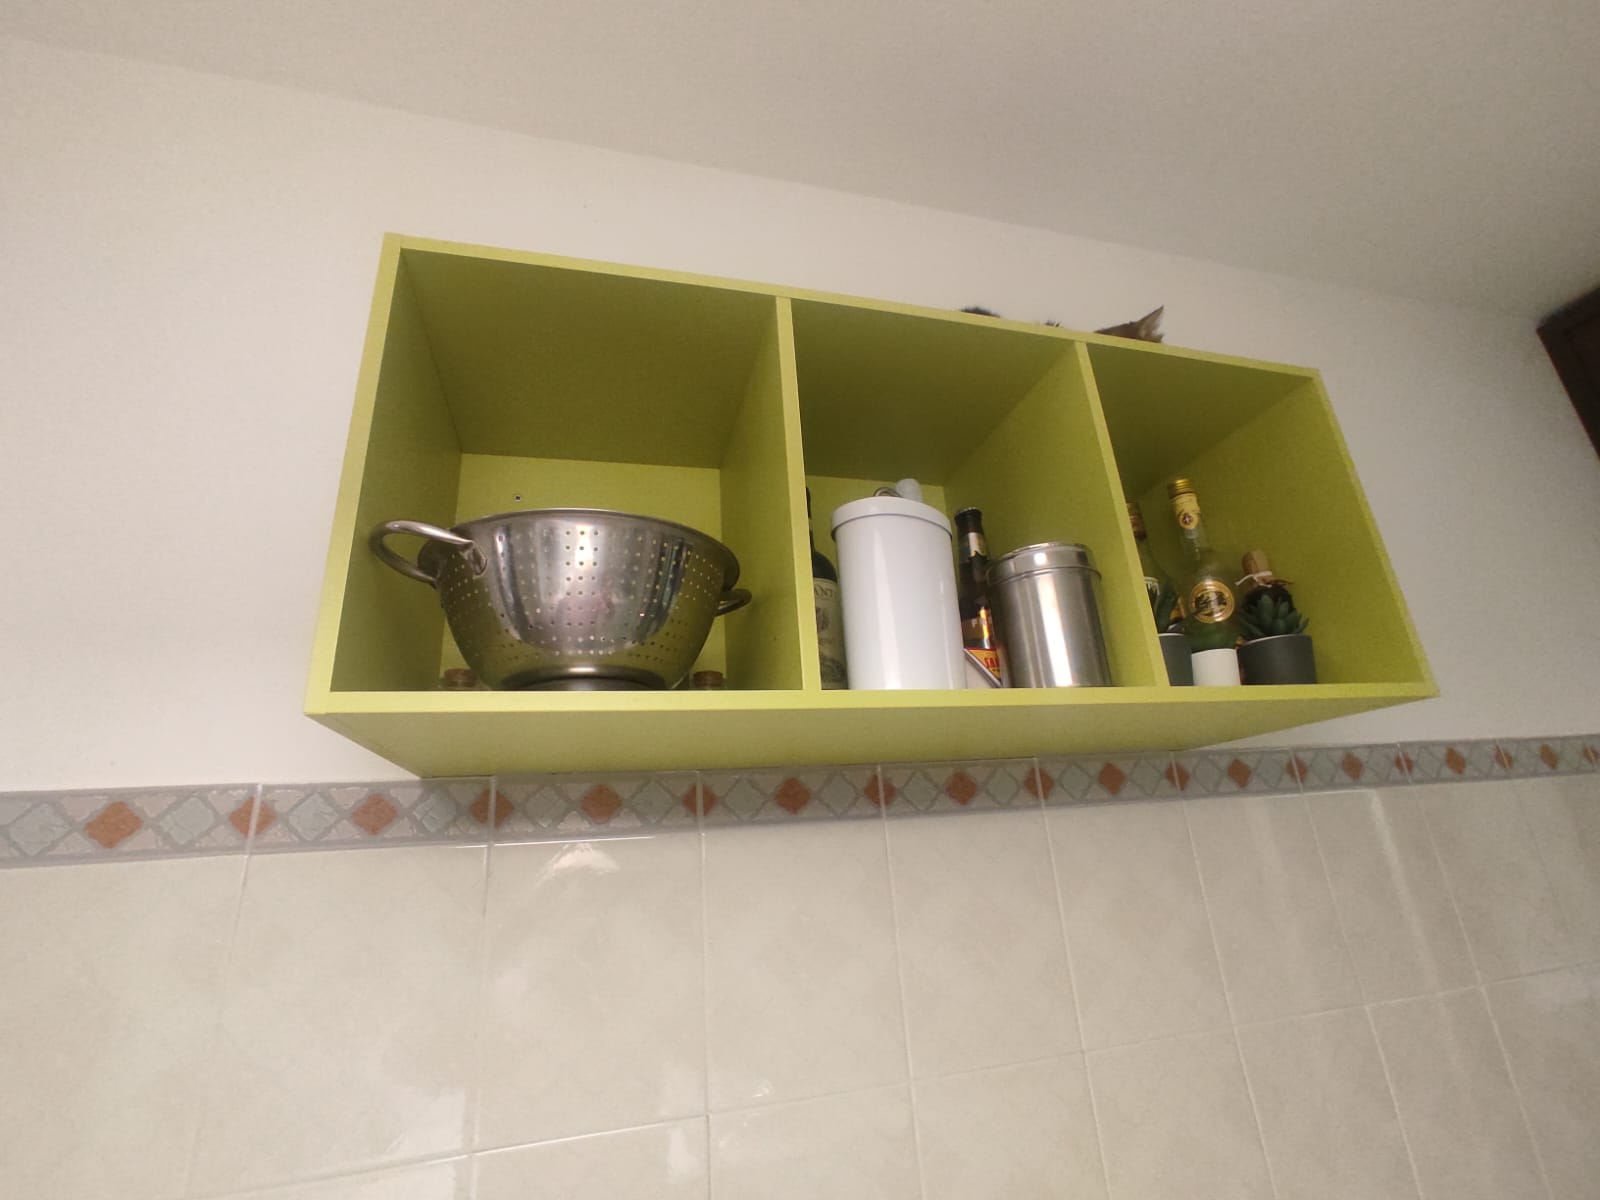
\includegraphics[width=1\textwidth]{homework.jpg}
    \end{figure}
\end{center}
\vspace{5mm}

\section{Theory}

\subsection{Question 1}

The vanishing line is the image of the line at infinity in the image horizontal plane. It is the connecting line of the two vanishing points of the image. The vanishing points are the points in the image where the parallel lines in the 3D world intersect.

It can be found, starting from the lines provided in the image, by finding the intersection point of the coplanar lines $l_2$, $l_3$ and $m_5$, $m_6$, and then finding the line connecting these two points.

All these operations can be computed via the cross product, exploiting the duality between points and lines in homogeneous coordinates.

\begin{equation*}
    vp_l = l_2 \times l_3
\end{equation*}
\begin{equation*}
    vp_m = m_5 \times m_6
\end{equation*}
\begin{equation}
    \mathbf{l'_\infty} = vp_l \times vp_m
\end{equation}

For the sake of numerical stability, it is better to normalize the vanishing line by its third entry. $l'_\infty = l'_\infty / {l'_\infty}_3$

\subsection{Question 2}

In order to find the Euclidean transformation, we must first find the image of the conic dual to circular points ${C^{*}_\infty}'$.

To do so, we can find the images of the circular points of the horizontal planes by intersecting the line $l'_\infty$ with the image of che conic $C$

\begin{equation}
    \begin{cases}
        \begin{bmatrix}
            x & y & 1
        \end{bmatrix}
        \begin{bmatrix}
            a_C   & b_C/2 & d_C/2 \\
            b_C/2 & c_C   & e_C/2 \\
            d_C/2 & e_C/2 & f_C
        \end{bmatrix}
        \begin{bmatrix}
            x \\ y \\ 1
        \end{bmatrix}
        = 0 \\
        {l'_\infty}^T
        \begin{bmatrix}
            x \\ y \\ 1
        \end{bmatrix}
        = 0
    \end{cases}
    \label{eq:conic}
\end{equation}

The quadratic system~\ref{eq:conic} will give us two (complex, since the conic and the line don't intersect) solutions, which are the images of the circular points of the horizontal plane $I', J'$.

The equation of the dual conic to the circular points is given by the equation

\begin{equation}
    {C^{*}_\infty}' = I' {J'}^T + {I'}^T J'
\end{equation}

Once we have found the image of the conic, we can find the Euclidean transformation $H_R$ matrix via the SVD decomposition of ${C^{*}_\infty}'$:

\begin{equation*}
    svd({C^{*}_\infty}')
    = H_R^{-1} \cdot C^{*}_\infty \cdot H_R^{-T} =
\end{equation*}
\begin{equation*}
    = U
    \begin{bmatrix}
        a & 0 & 0 \\
        0 & b & 0 \\
        0 & 0 & 0
    \end{bmatrix}
    U^T =
\end{equation*}
\begin{equation*}
    = U
    \begin{bmatrix}
        \sqrt{a} & 0        & 0 \\
        0        & \sqrt{b} & 0 \\
        0        & 0        & 1
    \end{bmatrix}
    \begin{bmatrix}
        1 & 0 & 0 \\
        0 & 1 & 0 \\
        0 & 0 & 0
    \end{bmatrix}
    \begin{bmatrix}
        \sqrt{a} & 0        & 0 \\
        0        & \sqrt{b} & 0 \\
        0        & 0        & 1
    \end{bmatrix}
    U^T
\end{equation*}
\begin{equation}
    \Rightarrow \mathbf{H_R} = \begin{bmatrix}
        \frac{1}{\sqrt{a}} & 0                  & 0 \\
        0                  & \frac{1}{\sqrt{b}} & 0 \\
        0                  & 0                  & 1
    \end{bmatrix}
    U^T
\end{equation}

After applying the transformation to the image, we can find the scale of the horizontal plane by measuring the length in pixes of $l_2$, using the standard formula for the distance between the two segment ends:

\begin{equation*}
    A = l_2 \times m_6 \quad B = l_2 \times l_5
\end{equation*}
\begin{equation*}
    A = A / A_3 \quad B = B / B_3
\end{equation*}
\begin{equation}
    Scale = \frac{1}{\sqrt{(A_1 - B_1)^2 + (A_2 - B_2)^2}}
\end{equation}

\noindent And find the actual length of the depth of the shelf (e.g. the length of $m_5$)
\begin{equation*}
    C = m_5 \times l_3
\end{equation*}
\begin{equation*}
    ||m_5||_{px} = \sqrt{(C_1 - B_1)^2 + (C_2 - B_2)^2}
\end{equation*}
\begin{equation}
    \mathbf{||m_5||_{real}} = ||m_5||_{px} \cdot Scale
\end{equation}

\subsection{Question 3}

To find the calibration matrix $K$, we can use also the vanishing point of the plane perpendicular to the horizontal plane

\begin{equation}
    vp_h = h_1 \times h_4
\end{equation}

\noindent Before going on, we need to define some useful notations:

\begin{equation}
    H = H_R^{-1} = [ch_1 \quad ch_2 \quad ch_3]
\end{equation}

\noindent And we can impose 4 independent constraints on the image of the absolute conic $\omega$

\begin{equation}
    \begin{cases}
        ch_1^T \cdot \omega \cdot ch_2 = 0                      \\
        ch_1^T \cdot \omega \cdot ch_1 - ch_2^T \omega ch_2 = 0 \\
        vp_h^T \cdot \omega \cdot ch_1 = 0                      \\
        vp_h^T \cdot \omega \cdot ch_2 = 0
    \end{cases}
\end{equation}

After solving for $\omega$, the calibration matrix $K$ can be found by the Cholesky decomposition of $\omega$:

\begin{equation}
    \omega = \mathbf{K} \cdot K^T
\end{equation}

\subsection{Question 4}

We can invert the previous computations to find the homography matrix $H_V$ that maps the vertical plane in the 3D world to the image vertical plane: this time, the unknowns are the (ratios of the) elements of the first two columns of $H_V$, so we need at least five constraints, including the orthogonality of the two columns:

\begin{equation*}
    H_V = [\xi_1 \quad \xi_2 \quad \xi_3]
\end{equation*}
\begin{equation}
    \begin{cases}
        \xi_1^T \cdot \omega \cdot \xi_2 = 0                                    \\
        \xi_1^T \cdot \omega \cdot \xi_1 - \xi_2^T \cdot \omega \cdot \xi_2 = 0 \\
        vp_m^T \cdot \omega \cdot \xi_1 = 0                                     \\
        vp_m^T \cdot \omega \cdot \xi_2 = 0                                     \\
        \xi_1^T \cdot \xi_2 = 0
    \end{cases}
\end{equation}

After solving for $\xi_1, \xi_2$, we can find the homography matrix $H_V$ by imposing the third column to be orthogonal to the first two:

\begin{equation}
    \xi_3 = \xi_1 \times \xi_2
\end{equation}

Now, we can find the rectifying homography matrix:

\begin{equation}
    H_{VR} = H_V^{-1}
\end{equation}

And computing the height of the parallelepiped $h$ in the 3D world exactly as we did for the depth of the shelf in question 2: finding the scale by measuring the length of $l_1$ in pixels in the rectified vertical plane, and then applying the proportion to the length of $h_1$ in pixels.

\subsection{Question 5}

To compute the X-Y coordinates of any point laying on any horizontal plane, we can use the standard formula of transformation of a point by means of the homography matrix $H$:

\begin{equation}
    x' = H \cdot x \Rightarrow \mathbf{x} = H^{-1} \cdot x' = H_R \cdot x'
\end{equation}

So, it is sufficient to apply the formula $H_R \cdot x'$ to every point extracted from the curve $S$ and, eventually, divide by the third coordinate to obtain the X-Y coordinates.

\subsection{Question 6}

To locate the parallelepiped, we need first to set the reference frame of the shelf (assuming the world frame is the same as the camera frame).

Without loss of generality, we can impose that the axis $x, y, z$ of the shelf reference frame are parallel respectively to the lines $l, m, h$ in the image.

After that, we can find the rotation and the translation of the parallelepiped by remembering the relation

\begin{equation*}
    H = K[r_x \quad r_y \quad t]
\end{equation*}
\begin{equation}
    \Rightarrow [\mathbf{r_x \quad r_y \quad t}] = K^{-1} \cdot H
\end{equation}

Where $r_x, r_y$ are the rotation of the axis $x, y$ of the shelf reference frame with respect to the camera frame, and $t$ is the translation of the origin of the shelf reference frame with respect to the camera frame.\\
The rotation $r_z$ can be found by knowing that the axis $z$ of the shelf reference frame is orthogonal to the plane of the shelf:

\begin{equation}
    \mathbf{r_z} = r_x \times r_y
\end{equation}

\vspace{2cm}

\section{Matlab}

\textit{Note:} all the outputs are also available in the \texttt{output} folder. In this section, I will comment them.\\
For completeness, I will also put the full Matlab output in the appendix.

\subsection{Problem 1}

Even if the image has been taken from a pinhole camera, there is still a little radial distortion in the image, resulting in non-perfect straight lines, as shown in Figure~\ref{fig:distortion}.

\begin{figure}[H]
    \centering
    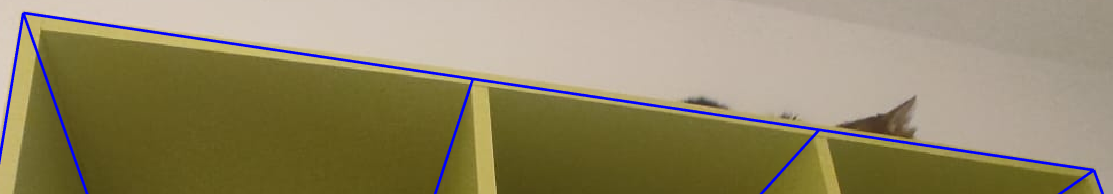
\includegraphics[width=1\textwidth]{output/distortion.png}
    \caption{Distortion in the image}
    \label{fig:distortion}
\end{figure}

To avoid problems in the computation of straight lines starting from the image, I have opted for corners detection techniques, using both the Harris corner detector and the FAST corner detector. The results are shown in Figure~\ref{fig:corners_detected}: red crosses are the corners detected by the Harris detector, while green crosses are the corners detected by the FAST detector\footnote{See \texttt{doDetection.m} script for all the steps followed}.

\begin{figure}[H]
    \centering
    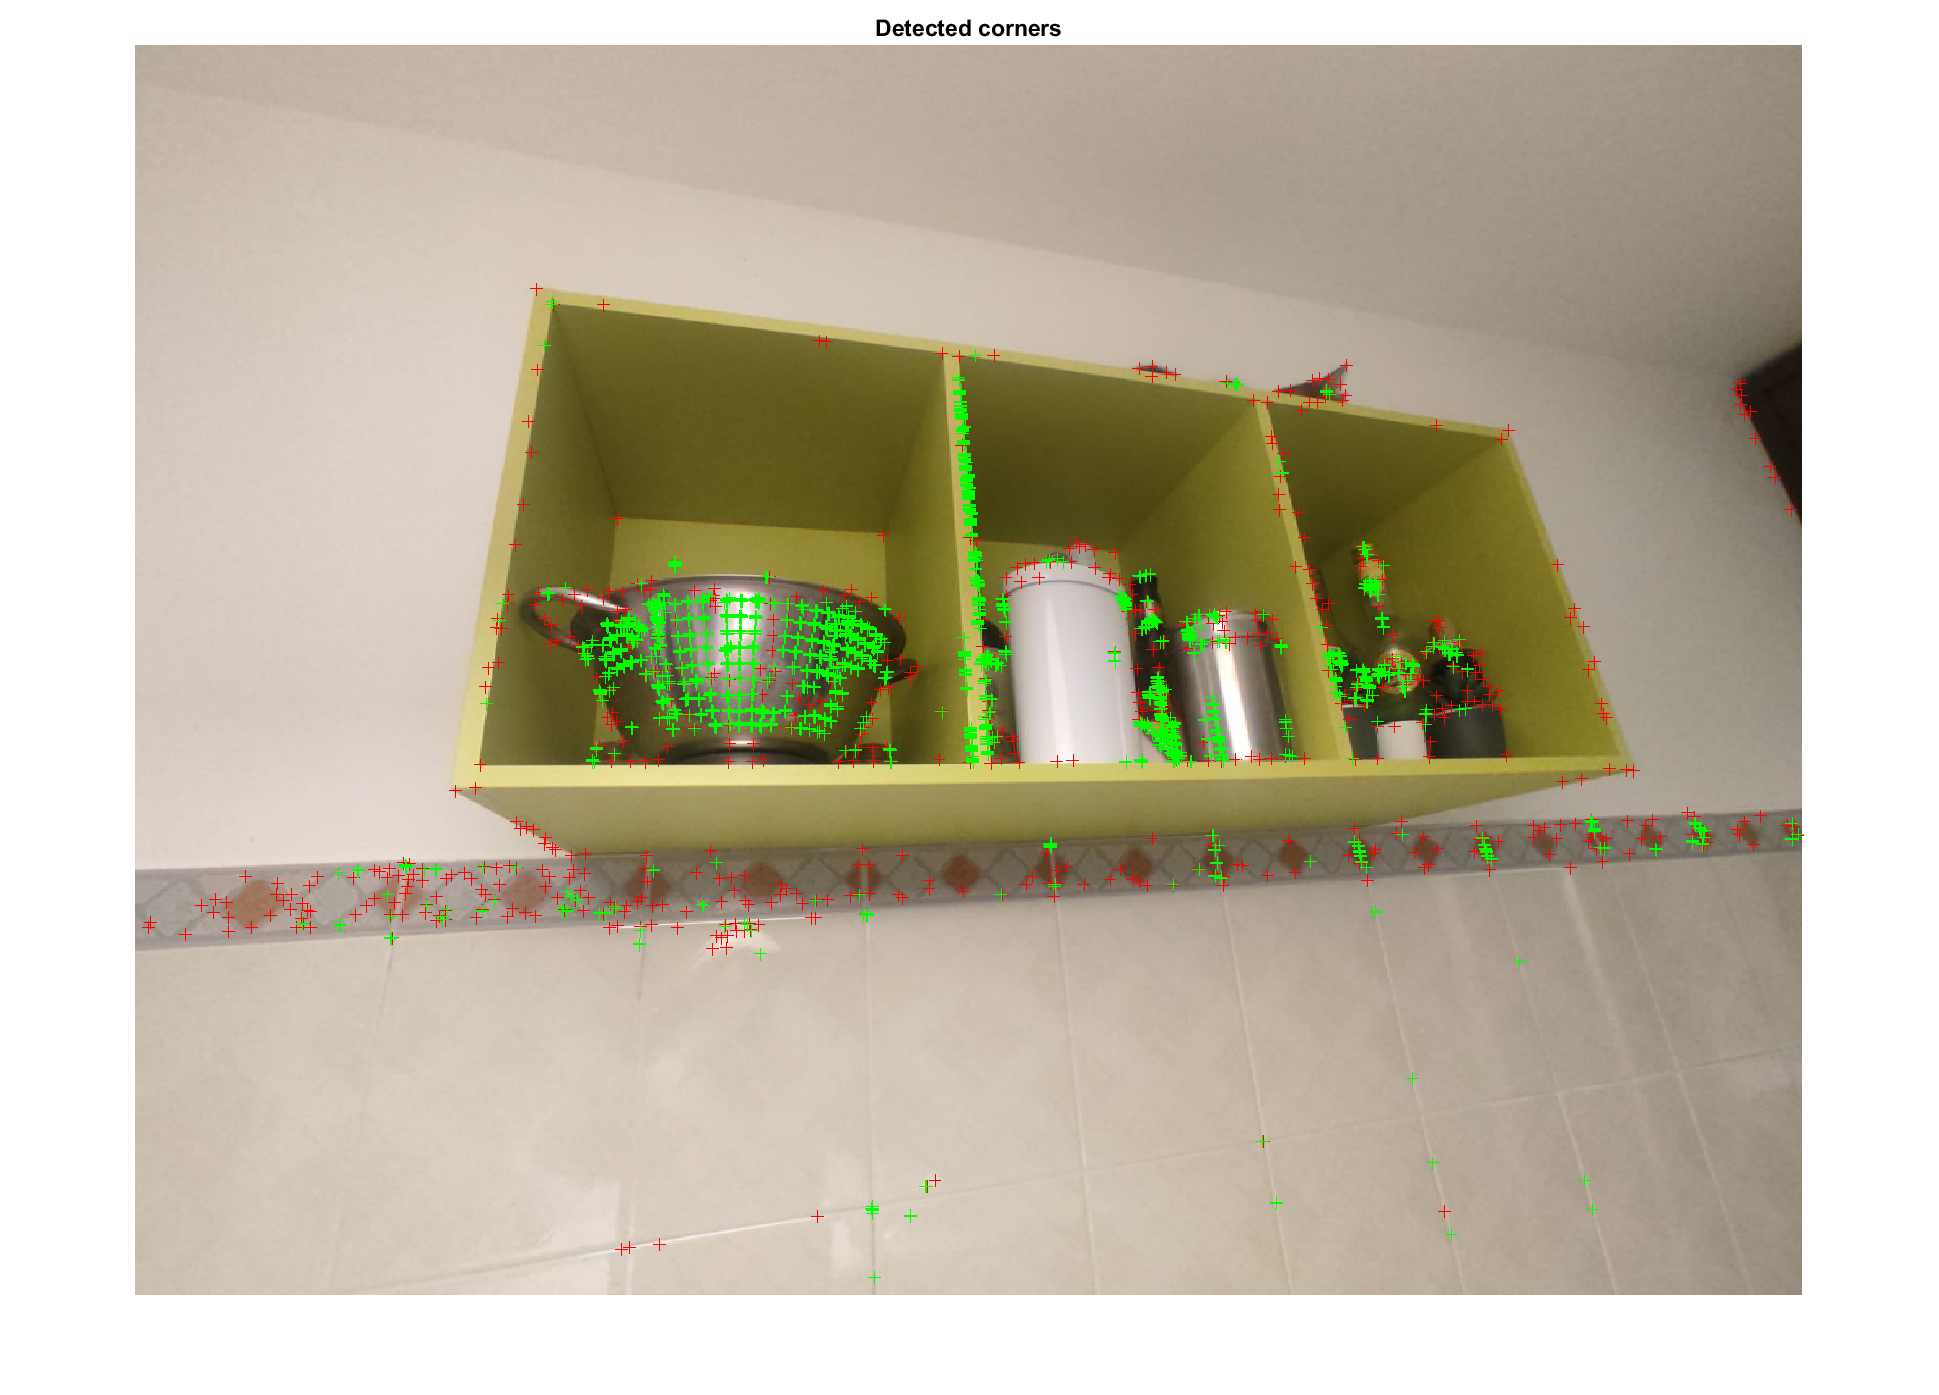
\includegraphics[width=.75\textwidth]{output/corners_detected.png}
    \caption{Detected corners}
    \label{fig:corners_detected}
\end{figure}

Once the corners have been detected, I manually selected all the corner relevant to the problem, and I computed the given lines. The results are shown in Figure~\ref{fig:lines_extracted}.

\begin{figure}[H]
    \centering
    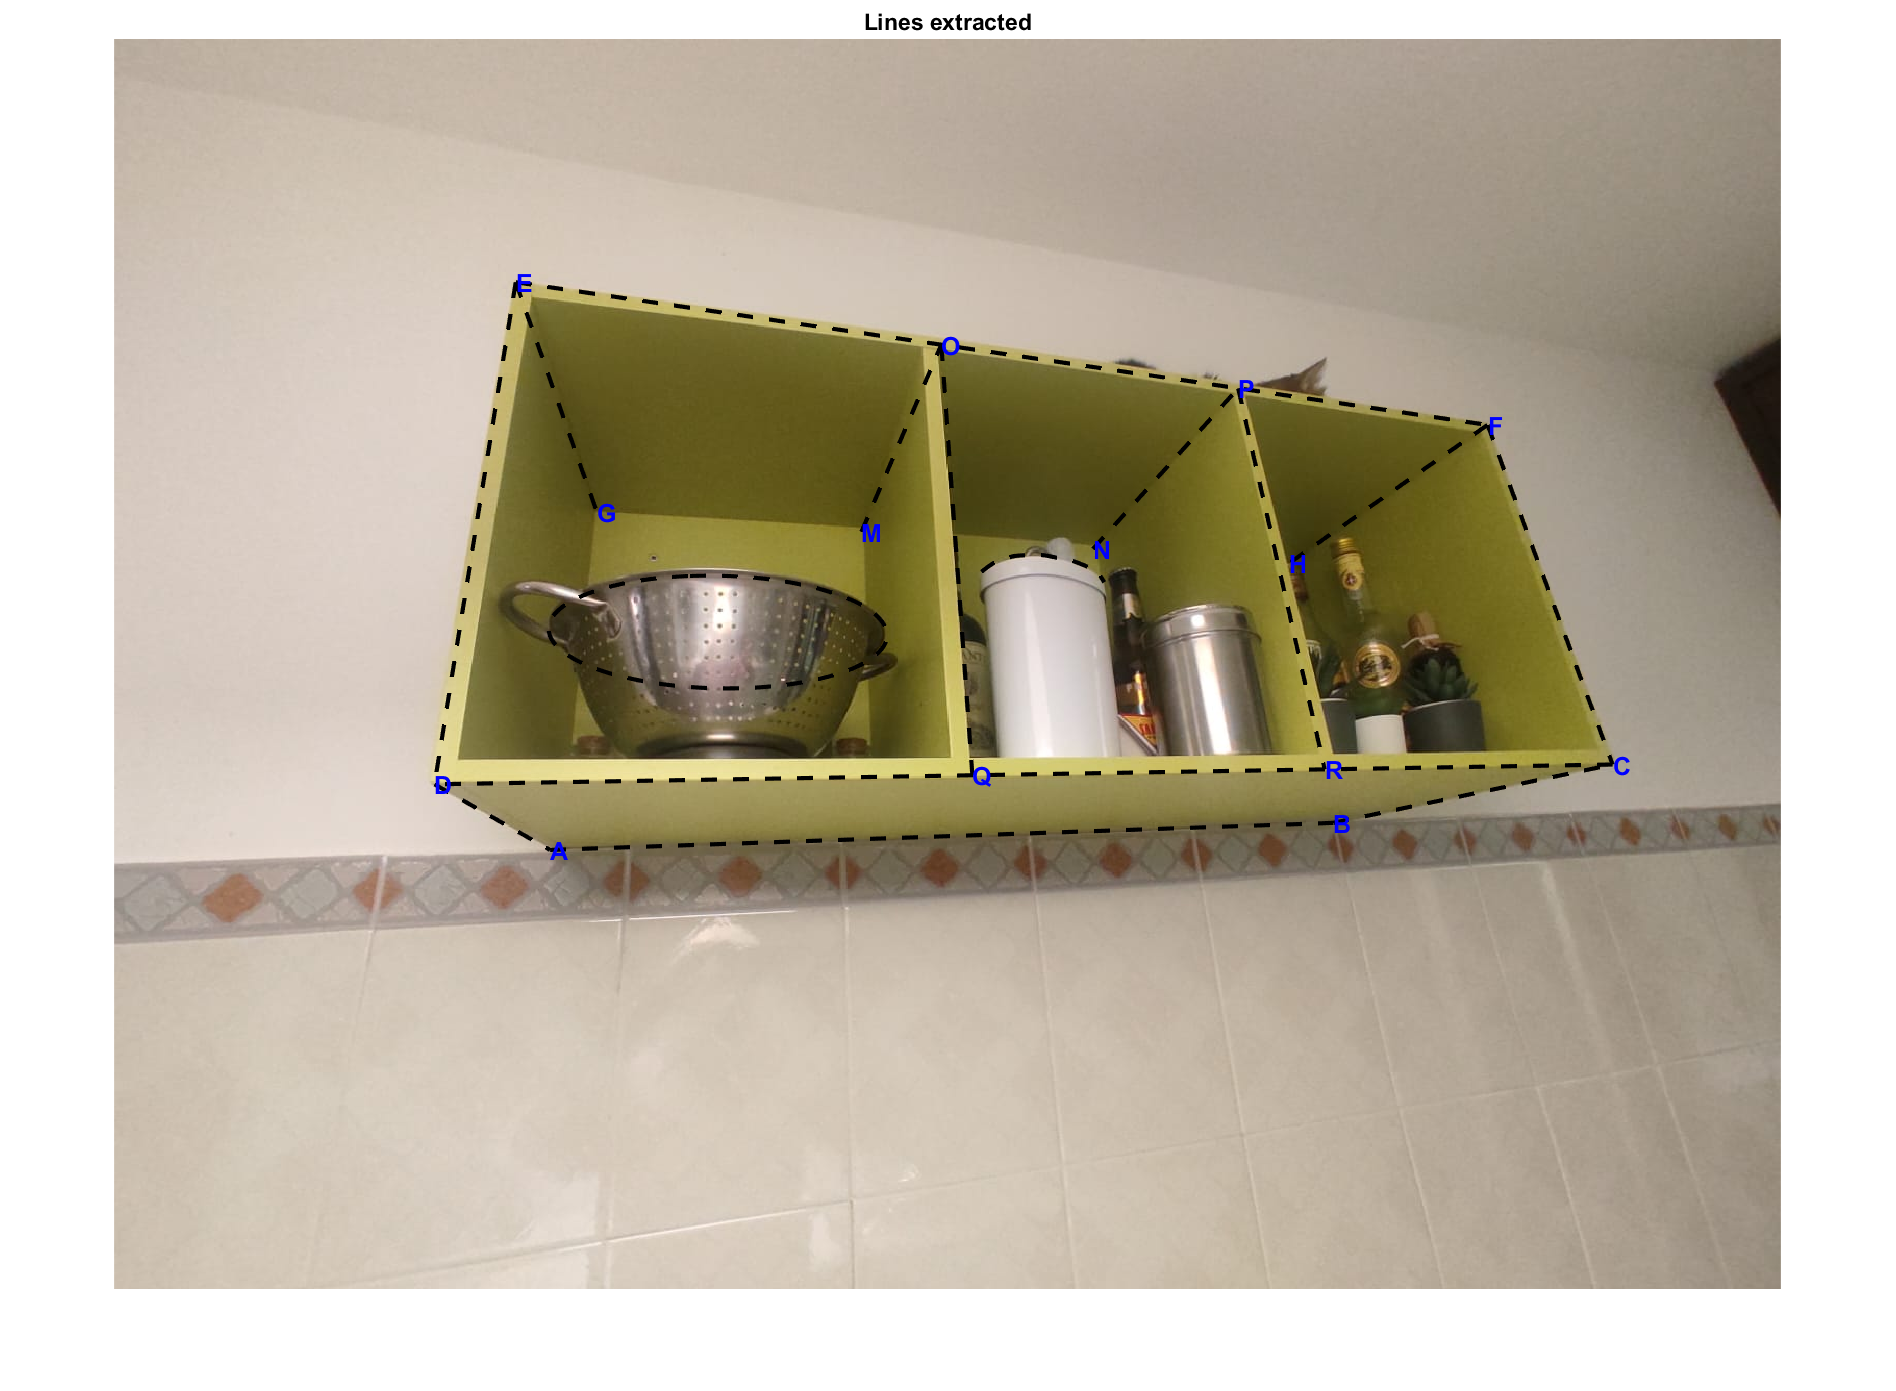
\includegraphics[width=.8\textwidth]{output/img_with_extracted_lines.png}
    \caption{Extracted lines, with named points}
    \label{fig:lines_extracted}
\end{figure}

During this process, the most challenging part was to obtain a sufficient number of points for the curve $S$, so I had to lower the threshold of the two detectors to get more points.

\subsection{Problem 2}

All the problems explained in the theory section have been solved following the steps described\footnote{See \texttt{homework.m} script for all the steps followed}.

\noindent Just a couple of notes about the script:
\begin{itemize}
    \item I have named the intersection points of the straight lines according to Figure~\ref{fig:lines_extracted} to make the code more readable and easier to debug.
    \item Every time an homography matrix was computed, the rectification of the whole image was quite challenging and the result was not always comprehensible~\ref{fig:failed_rec}, so, as a visual check, I performed the rectification of the corners belonging to the interested plane, and I plotted them in the image to check that the reconstructed shape was actually a rectangle. Examples are shown in Figure~\ref{fig:rectified_rects}.
    \item As a check for the correctness of the computations, I have also plotted the computed vanishing points, found during questions 1 and 3, in the image. The results are shown in Figure~\ref{fig:vanishing_points}.
    \item By visually inspecting the image, it appears that the depth and height of the shelf are approximately equal ($m \approx h$), and its length is roughly three times its height. These observations were validated by the computations.
\end{itemize}

\begin{figure}[H]
    \centering
    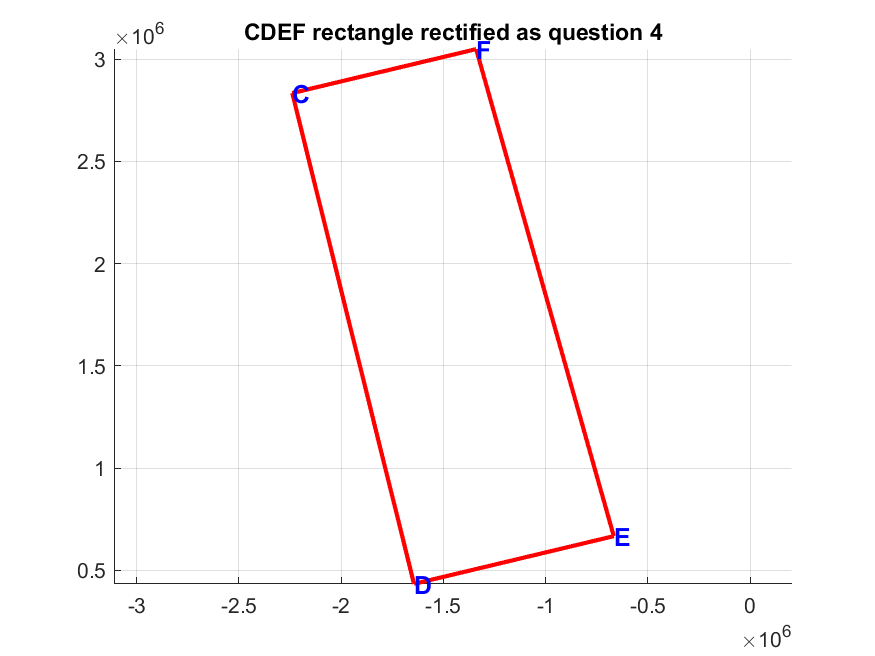
\includegraphics[width=.49\textwidth]{output/rectified_CDEF.png}
    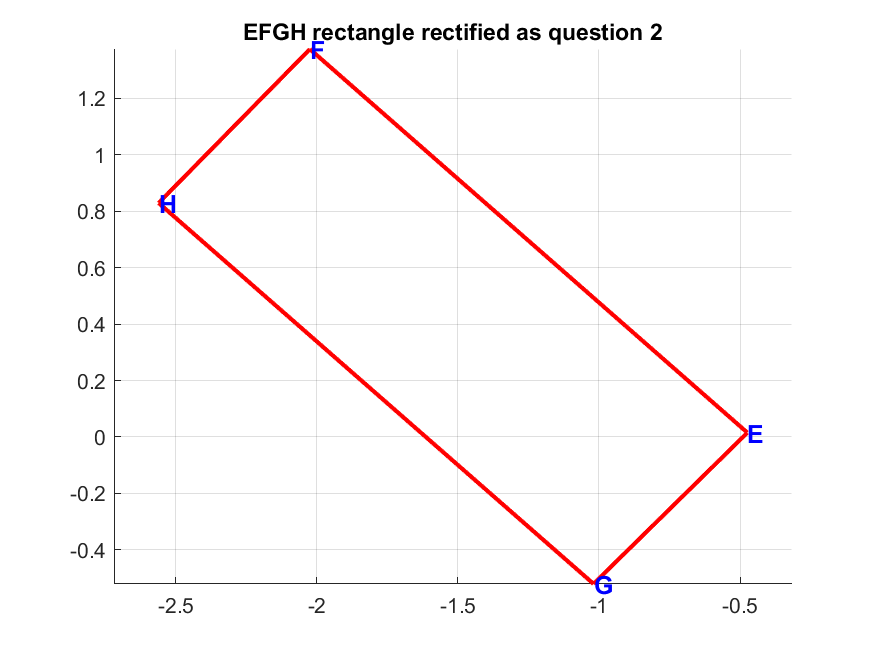
\includegraphics[width=.49\textwidth]{output/rectified_EFGH.png}
    \caption{Rectified rectangles from the computations of questions 2 and 4}
    \label{fig:rectified_rects}
\end{figure}

\begin{figure}[H]
    \centering
    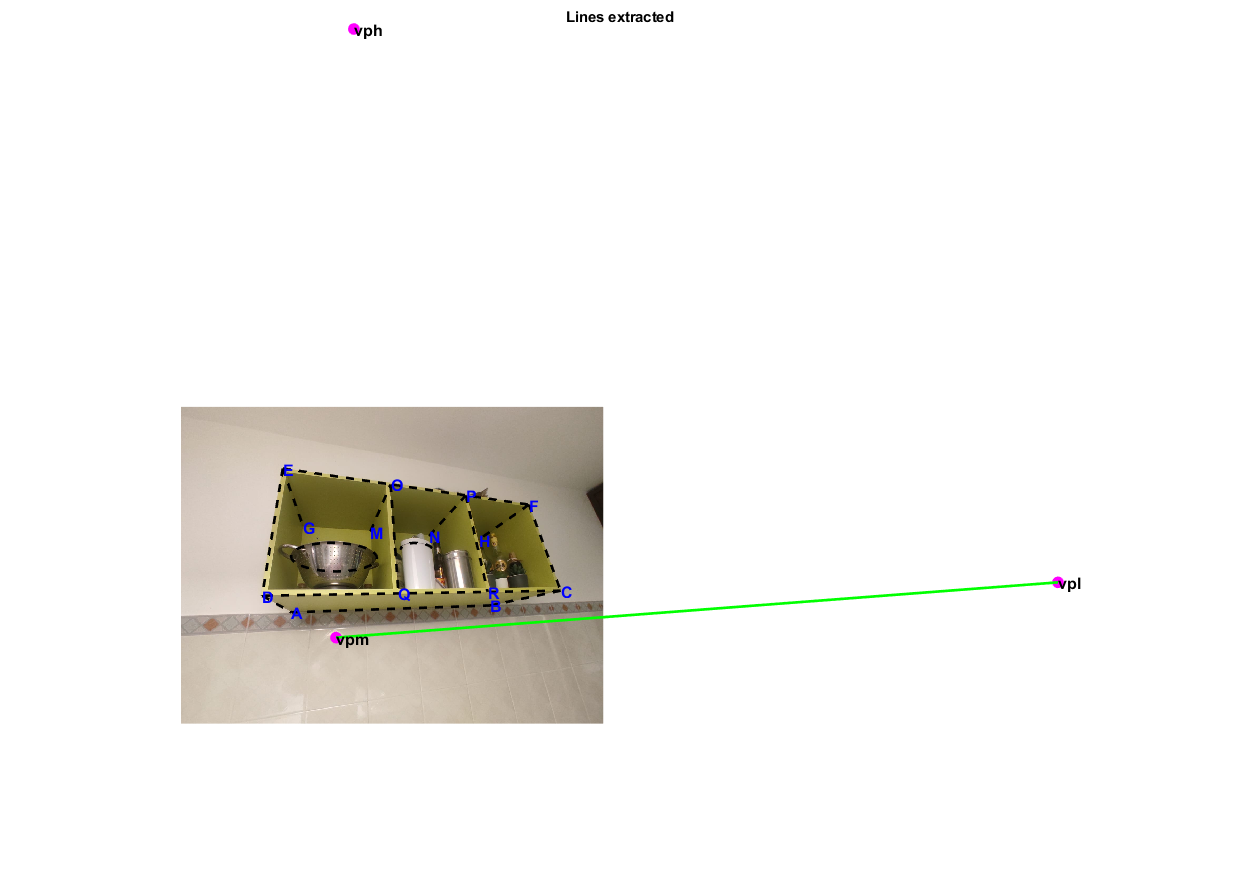
\includegraphics[width=.8\textwidth]{output/img_with_lines_and_vp.png}
    \caption{Vanishing points in the image}
    \label{fig:vanishing_points}
\end{figure}

\begin{figure}[H]
    \centering
    
\includegraphics[width=.5\textwidth]{output/rectified_img.png}
    \caption{Failed rectification of the whole image}
    \label{fig:failed_rec}
\end{figure}

\subsection{Problem 3}

When it came to the plot of the curve $S$\footnote{See \texttt{finalPlots.m} for the full script}, I interpolated the points with a cubic spline, and I plotted the curve in the image. The result is shown in Figure~\ref{fig:curve_S}.

\begin{figure}[H]
    \centering
    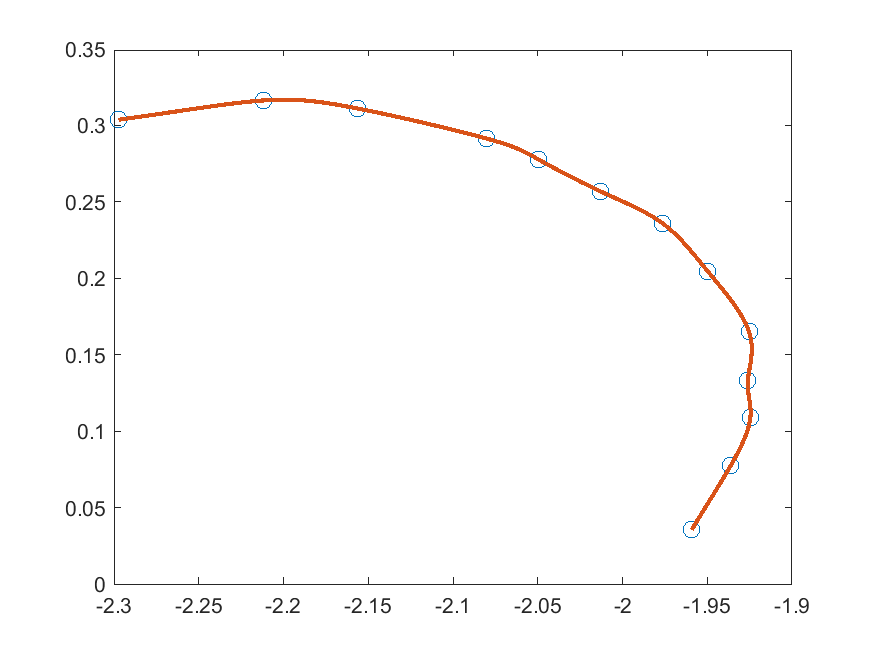
\includegraphics[width=.5\textwidth]{output/rectified_curve_S.png}
    \caption{Curve $S$ in the image}
    \label{fig:curve_S}
\end{figure}

As it can be seen, the curve is not perfectly regular, and this can be due to the fact that the points were not perfectly detected by the corner detectors, and the spline interpolation makes this imperfection more evident.


While for the 3D views of the shelf, I have computed the distance of the points $O,P$ from $E$ to correctly place the segments $h_2,h_3,m_2,m_3$ in the shelf. If I had computed the precise relative positions of all the points $M,N,Q,R$ with respect to $G,D$ and then matched them, the result would have been more coherent with the corners extracted before, but the difference would have been minimal and in my way the computations were cleaner.

To give a little of context to the 3D view, I have also plotted a circumference in a position similar to the position of the curve $C$. This was not computed, but helps to better visualize the 3D view of the shelf.

The final result is shown in Figure~\ref{fig:3D_shelf}.

\begin{figure}[H]
    \centering
    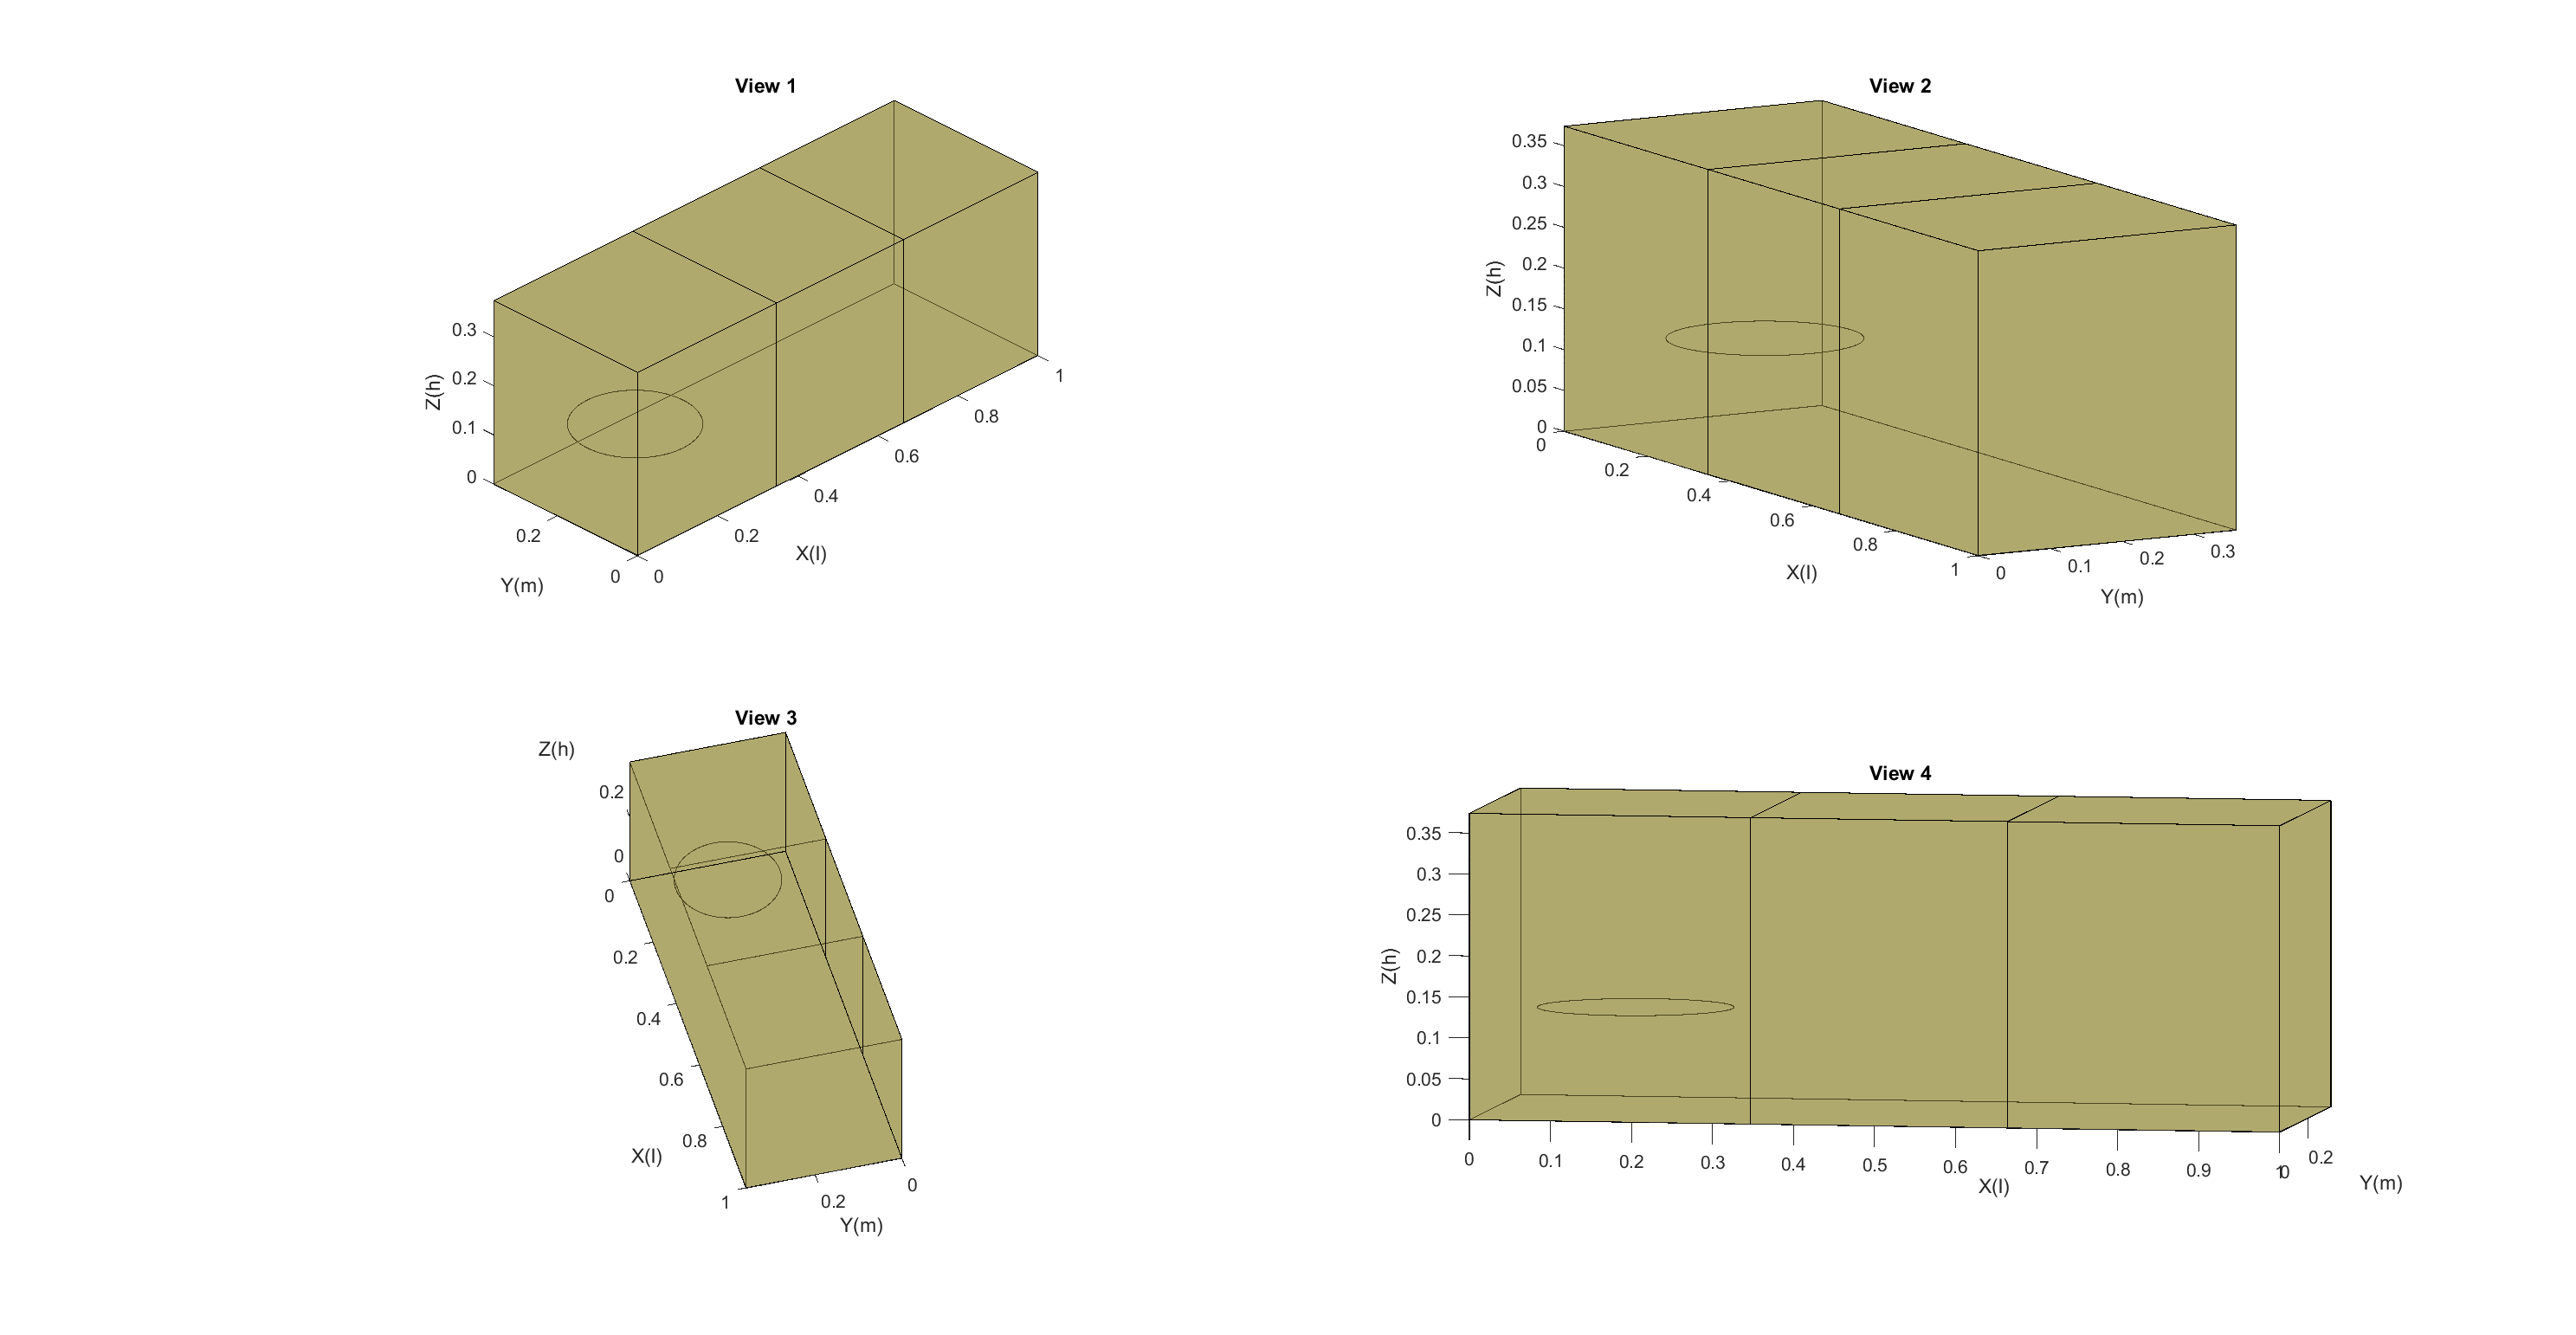
\includegraphics[width=.85\textwidth]{output/final_problem.png}
    \caption{3D view of the shelf}
    \label{fig:3D_shelf}
\end{figure}

\appendix

\section*{Matlab output}
\small{\texttt{\lstinputlisting[breaklines=true]{output/matlab_results.txt}}}

\end{document}